%Projects
%--------
%
%An essential part of this course are the take-home projects.
%
%Instructions for the take-home exams:
%
% Reports can be done individually or in groups of two. However, reasonably open
% discussions of the assignments with other students in this course are
% acceptable, but must be acknowledged in the report. The reports should consist
% of two to five pages plus supplementary graphs, tables, program listings, etc.,
% and should be organized as follows:
%
% Introduction and Problem Background. Briefly describe the general problem you
% want to solve and why a numerical or computational solution (as opposed to an
% exclusively analytical solution) is required.
%
% Numerical Considerations. Briefly discuss the specific methods, software or
% algorithms you selected for this problem. Mention any specific features of
% MATLAB you exploited.
%
% Results.  Include a concise tabular or graphical presentation of the results.
% Every table and figure should have a caption and a title, and the axes of every
% plot should be clearly marked, so that the reader can understand the figures or
% plots without referring to the main text. All codes should be clearly
% documented, especially input and output parameters, if any, and a description
% of what the code does.
%
% Analysis. Include a solid discussion and analysis of the results presented.
% The discussion should address any difficulties you encountered, appropriate
% measures of performance (such as errors and computer time) and the apparent
% sources of error you observed.
%
% Lessons Learned. Elaborate a critical evaluation of the software you used. Make
% a list of the specific things you  learned by working out the assignment, both
% theoretical and practical issues.
%
% Acknowledgements. Mention discussions with other students or teachers, software
% downloaded from the web or  copied from a book, and any other relevant
% information you find fit to disclose.
%
% The grade you obtain will reflect whether or not you have correctly and
% efficiently solved the problem, and whether or not you adequately address the
% relevant theoretical and practical issues. A grade of 8-12 indicates work that
% is acceptable, contains only minor errors, but is otherwise unexceptional. A
% grade of 13-15 indicates work that is correct, especially efficient and well
% documented, addresses all the points mentioned above, and contains unusually
% clear outputs and a serious and thorough analysis of those outputs.
%
% The report may be written in Swedish or English. Include name(s), ID number(s)
% and e-mail(s).
%
% Please hand in the report on paper (not via e-mail) at a lecture or seminar, or
% else place it in the box marked FMNF05 at the bottom of the shelf located at
% the entrance of the right-hand side corridor (MH, ground floor). The first
% report will be collected at 12:00 on Feb 2, 2018. The second project will be
% collected at 12:00 on Feb 23, 2018. Any report handed in or placed in the box
% after this time will not be accepted.

\documentclass{article}

\usepackage[utf8]{inputenc}
\usepackage[T1]{fontenc}
\usepackage{gensymb}
\usepackage{amsmath}
\usepackage{graphicx}

\begin{document}

\begin{center}
  {\small FMNF05 - Computational Project 1} \\
  {\Large\textbf{Numerical Crime Scene Investigation}} \\
  \vspace{0.4cm}
  \today\\
  \vspace{0.2cm}
  Stefan Eng \texttt{<atn08sen@student.lu.se>} \\
  \vspace{0.4cm}
  {\Large ---} \\
\end{center}

\section*{Introduction}

The problem consists of determining when Professor Bill Grimssom was
murdered by calculating at which time ($t_d$) the body had a temperature of
37.0{\degree}C. This information is needed in order to check if the alibi
stated by the suspected inspector Sutherland is good enough. The reason the
problem can't be analytically solved is that there are computations (shown
later) that include trancendental numbers which will need to be approximated.

\subsection*{Problem data}

  $T_{body}(\textrm{20:00}) = 32.0{\degree}C = T_{body}(0)$\\
  $T_{body}(\textrm{21:00}) = 29.5{\degree}C = T_{body}(1)$\\
  $T_{body}(t_{death}) = 37.0\degree{C} $ \\

  \noindent
  $T_{office}(\textrm{16:00}) = 22.0{\degree}C = T_{office}(0) $\\
  $T_{office}(t) = 22.0{\degree}C + 0.5{\degree}C \cdot t $ \\

  \noindent
  Newtons law of cooling, $k$ = positive constant of proportionality: \\
  $T_{body}'(t) = -k(T_{body}(t) - T_{office}(t))$

\section*{Numerical Considerations}

MATLAB is the software used to preforme the calculations needed to complete the
project. In order to approximate necessary koefficients and roots the following
algoritmic methods were used and compared; \textit{bisection}, \textit{fixed-point} and
\textit{Newton-Raphson}. As part of the final analysis of the other methods
the built-in MATLAB-function \textit{fzero} was used to compare reults.

\section*{Results}

  \textbf{Task 1:}
  Show that
  $T_{body}(t) = 22 + 0.5t - \frac{1}{2k} + c\mathrm{e}^{-kt}$ is a solution to
  \\
  $T_{body}'(t) = -k(T_{body}(t) - T_{office}(t))$
  given:
  $T_{office}(t) = 22.0{\degree}C + 0.5{\degree}C \cdot t $. \\

  \noindent
  Taking the derivative of the given $T_{body}$ solution and using it in the
  Newtons law of cooling results in the equations:
  %$T_{body}(t) = 22 + 0.5t - \frac{1}{2k} + c\mathrm{e}^{-kt}$ \\
  %$T_{body}'(t) = 0.5 -kc\mathrm{e}^{-kt}$ \\

  \noindent
  \begin{align*}
%    T_{body}'(t) &= -k(T_{body}(t) - T_{office}(t)) \\
    0.5 -kc\mathrm{e}^{-kt} &= -k(22 + 0.5t - \frac{1}{2k} + c\mathrm{e}^{-kt}
    - 22 - 0.5t) \\
    0.5 -kc\mathrm{e}^{-kt} &= -k(-\frac{1}{2k} + c\mathrm{e}^{-kt}) \\
    0.5 -kc\mathrm{e}^{-kt} &= 0.5 - kc\mathrm{e}^{-kt}
  \end{align*}


  \noindent
  Which proves that the given solution is correct. \\

%\section*{Task 2}

  \noindent
  \textbf{Task 2.1:}
  Show that using the known $T(0) = 32.0$ data-point results in the equation:
  $T(t) = 22 + 0.5t - \frac{1}{2k} + (10 + \frac{1}{2k})\mathrm{e}^{-kt}$. \\

  \noindent
  Using the solution from above and $t=0$ results in the follwing equation:
  \begin{align*}
%    T_{body}(t) &= 22 + 0.5t - \frac{1}{2k} + c\mathrm{e}^{-kt} \\
    T_{body}(0) &= 22 - \frac{1}{2k} + c\mathrm{e}^{0} \\
    32 &= 22 - \frac{1}{2k} + c \\
%    10 &= -\frac{1}{2k} + c \\
    c  &= 10 + \frac{1}{2k}
  \end{align*}

  \noindent
  Where substituting the value $c$ calculated above into
  $T(t) = 22 + 0.5t - \frac{1}{2k} + c\mathrm{e}^{-kt}$
  results in the sought after equation. \\

  \noindent
  \textbf{Task 2.2:}
  Show that using the data-point $T(1) = 29.5$ results in the following
  equation:
  $ 7 + \frac{1}{2k} = (10 + \frac{1}{2k})\mathrm{e}^{-k} $. \\

  \noindent
  As previously, use the proposed solution $T(t)$ with $t=1$ and obtain:

  \begin{align*}
%    T_{body}(t) &= 22 + 0.5t - \frac{1}{2k} + c\mathrm{e}^{-kt} \\
    T_{body}(1) &= 22 + 0.5 - \frac{1}{2k} + c\mathrm{e}^{-k} \\
    29.5 &= 22.5 - \frac{1}{2k} + c\mathrm{e}^{-k} \\
%    7 &= - \frac{1}{2k} + c\mathrm{e}^{-k} \\
    7 + \frac{1}{2k} &= (10 + \frac{1}{2k})\mathrm{e}^{-k}
  \end{align*}

  \noindent
  Which is the equation mentioned above. \\

  \noindent
  As an additional note, it is here that the possibility to solve the problem
  analytcally breakes down. Trying to solve the previous equation for $k$
  results in envaluating $\mathrm{ln}(\frac{7}{2})$ which is a trancendental
  number. \\

  \noindent
  \textbf{Task 3:}
  Construct a MATLAB algorithm that approximates the value of $k$ with an
  accuaracy of two decimal places using the bisection method. \\

  \noindent
  The task is equivalent to finding a root to the function:
  $ f(x) = 7 + 0.5x - (10 + 0.5x)\mathrm{e}^{-x} $.
  In order to use the bisection method, an intitial x-interval of $[a, b]$ must
  be choosen in such a way that $f(a) * f(b) < 0$, i.e. the interval brackets the
  root. Two such values are 0 and 1, which results in; $f(0) = -3$ and $f(1) >
  0$, which gives the initial values of $a=0$ and $b=1$.

  \begin{center}
    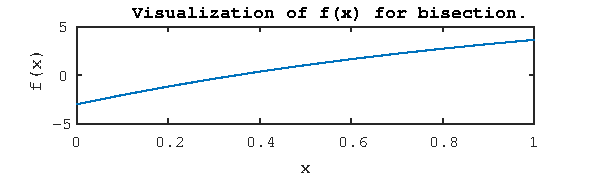
\includegraphics{figs/t3_check.pdf}
  \end{center}

  \noindent
  Here is the bisection MATLAB code:

  \begin{verbatim}
function [xc, iters, errors] = bisection(f, a, b, eps, Nmax)
  % Calculate function values based on inverval.
  fa = f(a); fb = f(b);
  iters = 1;
  errors = [];
  while iters <= Nmax
    % Claculate error and append to errors array.
    err = (b-a)/2;
    errors(end+1) = err;
    % Break if eps is satisfied.
    if err < eps; break; end
    % Caculate new mid and function value.
    mid = (a+b)/2; fmid = f(mid);
    % Break if fmid is a root.
    if fmid == 0; break; end
    % Not root, construct new interval.
    if fa * fmid < 0 % [a, mid] includes root.
      b = mid;
    else % [mid, b] includes root.
      a = mid; fa = fmid;
    end
    iters = iters + 1;
  end
  % Calculate and return approximate root.
  xc = (a+b)/2;
end
  \end{verbatim}

  \noindent
  Running the $k_c =\ $\texttt{bisection} in MATLAB, with $a=0$, $b=1$,
  $\epsilon=0.5*10^{-2}$ and $Nmax=100$, produces $k_c = 0.34961$ with $f(k_c) =
  0.001940 \ ( < 0.5*10^{-2} )$ running 9 iterations.\\

  \noindent
  \textbf{Task 4:}
  Use a algorithm based on the fixed point method to appriximate
  $k$ to 6 decimal accuracy.
  \begin{align*}
     f(x) &= 7 + 0.5x - (10 + 0.5x)\mathrm{e}^{-x} = 0\\
     0  &= 7 + 0.5x - (10 + 0.5x)\mathrm{e}^{-x} \\
     - 0.5x  &= 7 - (10 + 0.5x)\mathrm{e}^{-x} \\
     x  &= -2(10 + 0.5x)\mathrm{e}^{-x} + 14  = g(x)
  \end{align*}

  \noindent
  $ g(x) = -2(10 + 0.5x)\mathrm{e}^{-x} + 14 $ \\
  $ g(x) = -20\mathrm{e}^{-x} - x\mathrm{e}^{-x} + 14 $ \\
  $ g'(x) = \mathrm{e}^{-x}(19 + x)$ \\

  \noindent
  Plugging in $k_c$ from the previous computation results in:  $|g'(k_c)| = |14.35|
  > 1 $, which indicates that the fixed-point iteration will not converge.
  Rewriting $g(x)$ in the the following way:

  \noindent
  \begin{align*}
    0  &= 7 + 0.5x - (10 + 0.5x)\mathrm{e}^{-x} \\
    -7 -0.5x  &= -(10 + 0.5x)\mathrm{e}^{-x} \\
    \mathrm{e}^{x}(-7 -0.5x)  &= -10 + 0.5x \\
    \mathrm{e}^{x}  &= \frac{-10 + 0.5x}{-7-0.5x} \\
    g(x) &= \mathrm{ln}(\frac{-10 + 0.5x}{-7-0.5x})
  \end{align*}
  \noindent
  gives $|g'(k_c)| = |0.0429| < 1 $, which makes the fixed-point algorithm converge to
  $ k_c = 0.349345 $ in 3 iterations, with the result $f(k_c) =
  8.1904*10^{-7}$. \\

  \noindent
  MATLAB code for fixed-point:

  \begin{verbatim}
function [xc, iters, errors] = fixed_point(g, guess, eps, Nmax)
  iters = 1; xc = guess;
  errors = [];
  while iters <= Nmax
    nxc = g(xc);
    % Calculate difference between previous and current guess.
    err = abs(xc - nxc);
    % Append error to errors array.
    errors(end+1) = err;
    % Use current nxc value as next xc value.
    xc = nxc;
    % Break if new guess similar enough to previous guess.
    if err < eps; break; end
    iters = iters + 1;
  end
end
  \end{verbatim}

  \noindent
  \textbf{Task 5:}
  Use the appriximated value for $k$, $k_c$ and the Newton-Raphson method to
  calculate $T(t) = 37$ in order to determine the time of death. \\

  \noindent
  The body-temparture equation according to earlier with $k = k_c$:
  \begin{align*}
    T(t) &= 22 + 0.5t - 0.5k_c + (10 + 0.5k_c)\mathrm{e}^{-k_ct} \\
    37 &= 22 + 0.5t - 0.5k_c + (10 + 0.5k_c)\mathrm{e}^{-k_ct} \\
    f(t) &= -15 + 0.5t - 0.5k_c + (10 + 0.5k_c)\mathrm{e}^{-k_ct} \\
    f'(t) &=  0.5 -k_c(10 + 0.5k_c)\mathrm{e}^{-k_ct}
  \end{align*}

%  \noindent
%  Plotting the function $f(t)$ for different x-intervals results in the
%  follwing graphs:
%
%  \begin{center}
%    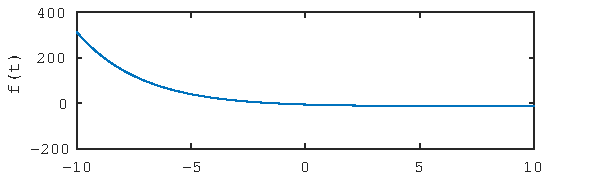
\includegraphics{figs/t5_check.pdf}
%  \end{center}
%
%  \begin{center}
%    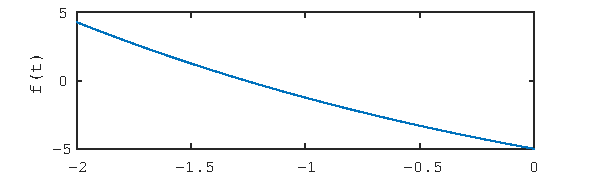
\includegraphics{figs/t5_check_2.pdf}
%  \end{center}

  \noindent
  Running Newton results in $t_d = -1.2607242282512758$, computed in 4
  iterations. \\

  \noindent
  MATLAB code:
  \begin{verbatim}
function [xc, iters, errors] = newtonraphs(f, fp, k, guess, eps, Nmax)
  iters = 1;
  xc = guess;
  errors = [];
  while iters <= Nmax
    nxc = xc - (f(xc, k)/fp(xc, k));
    err = f(nxc, k);
    errors(end+1) = err;
    iters = iters + 1;
    xc = nxc;
    if abs(err) < eps; break; end
  end
end
\end{verbatim}

  \noindent
  \textbf{Task 6:}
  Compute $t_d$ by using the other methods.

  \noindent
  Setting up fixed-point.
  \begin{align*}
    0 &= -15 + 0.5t - 0.5k_c + (10 + 0.5k_c)\mathrm{e}^{-k_ct} \\
  %  15 - 0.5t + 0.5k_c &= (10 + 0.5k_c)\mathrm{e}^{-k_ct} \\
  %  \frac{15 - 0.5t + 0.5k_c}{10 + 0.5k_c} &= \mathrm{e}^{-k_ct} \\
    \mathrm{ln}(\frac{15 - 0.5t + 0.5k_c}{10 + 0.5k_c}) * \frac{1}{-k} &= t \\
  \end{align*}

  \noindent
  Bisection method computed $(t_d)$ = -1.2607242282512758 in 52 iterations. \\
  Fixed-point method computed $(t_d)$ = -1.2607242282512761 in 15 iterations.

  \noindent
  (Tabluated values included last.)

 % \begin{center}
 %   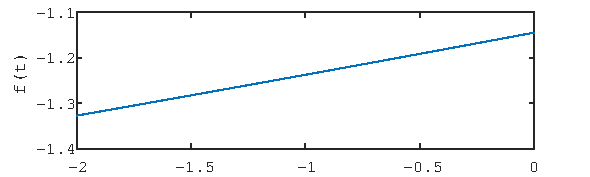
\includegraphics{figs/t6_check_1.pdf}
 % \end{center}

\noindent
\textbf{Task 7:}
Results are comparable.
\begin{verbatim}
Task7 -- Comapare to fzero results.
---
fzero solution for 	kc = 0.3493444395891339.
my solution for 	kc = 0.3493444415268486.
fzero solution for tc with my kc, 		tc = -1.2607242282512761.
fzero solution for tc with fsolve kc, 		tc = -1.2607242360472339.
\end{verbatim}

\noindent
\textbf{Task 8:}
He had time to do it later.

\section{Appendix}

\begin{verbatim}
Newton method:
--------------
i 	 e_i			e_i/e_{i-1}
0 	 0.0001110994570706
1 	 0.0000000004721112 	0.0000042494468600
2 	 0.0000000000000000 	0.0000000000000000

Bisection method:
-----------------
i 	 e_i			e_i/e_{i-1}
0 	 0.7500000000000000
1 	 0.3750000000000000 	0.5000000000000000
2 	 0.1875000000000000 	0.5000000000000000
3 	 0.0937500000000000 	0.5000000000000000
4 	 0.0468750000000000 	0.5000000000000000
5 	 0.0234375000000000 	0.5000000000000000
6 	 0.0117187500000000 	0.5000000000000000
7 	 0.0058593750000000 	0.5000000000000000
8 	 0.0029296875000000 	0.5000000000000000
9 	 0.0014648437500000 	0.5000000000000000
10 	 0.0007324218750000 	0.5000000000000000
11 	 0.0003662109375000 	0.5000000000000000
12 	 0.0001831054687500 	0.5000000000000000
13 	 0.0000915527343750 	0.5000000000000000
14 	 0.0000457763671875 	0.5000000000000000
15 	 0.0000228881835938 	0.5000000000000000
16 	 0.0000114440917969 	0.5000000000000000
17 	 0.0000057220458984 	0.5000000000000000
18 	 0.0000028610229492 	0.5000000000000000
19 	 0.0000014305114746 	0.5000000000000000
20 	 0.0000007152557373 	0.5000000000000000
21 	 0.0000003576278687 	0.5000000000000000
22 	 0.0000001788139343 	0.5000000000000000
23 	 0.0000000894069672 	0.5000000000000000
24 	 0.0000000447034836 	0.5000000000000000
25 	 0.0000000223517418 	0.5000000000000000
26 	 0.0000000111758709 	0.5000000000000000
27 	 0.0000000055879354 	0.5000000000000000
28 	 0.0000000027939677 	0.5000000000000000
29 	 0.0000000013969839 	0.5000000000000000
30 	 0.0000000006984919 	0.5000000000000000
31 	 0.0000000003492460 	0.5000000000000000
32 	 0.0000000001746230 	0.5000000000000000
33 	 0.0000000000873115 	0.5000000000000000
34 	 0.0000000000436557 	0.5000000000000000
35 	 0.0000000000218279 	0.5000000000000000
36 	 0.0000000000109139 	0.5000000000000000
37 	 0.0000000000054570 	0.5000000000000000
38 	 0.0000000000027285 	0.5000000000000000
39 	 0.0000000000013642 	0.5000000000000000
40 	 0.0000000000006821 	0.5000000000000000
41 	 0.0000000000003411 	0.5000000000000000
42 	 0.0000000000001705 	0.5000000000000000
43 	 0.0000000000000853 	0.5000000000000000
44 	 0.0000000000000426 	0.5000000000000000
45 	 0.0000000000000213 	0.5000000000000000
46 	 0.0000000000000107 	0.5000000000000000
47 	 0.0000000000000053 	0.5000000000000000
48 	 0.0000000000000027 	0.5000000000000000
49 	 0.0000000000000013 	0.5000000000000000
50 	 0.0000000000000007 	0.5000000000000000
51 	 0.0000000000000003 	0.5000000000000000

Fixed-point method:
-------------------
i 	 e_i			e_i/e_{i-1}
0 	 0.0552199521543004
1 	 0.0050057834598398 	0.0906517167173963
2 	 0.0004533504189319 	0.0905653275993714
3 	 0.0000410542837004 	0.0905575069216988
4 	 0.0000037177445056 	0.0905567987183748
5 	 0.0000003366668029 	0.0905567347015985
6 	 0.0000000304874441 	0.0905567280883654
7 	 0.0000000027608431 	0.0905567255287388
8 	 0.0000000002500131 	0.0905568014494763
9 	 0.0000000000226401 	0.0905556951896117
10 	 0.0000000000020504 	0.0905631509778153
11 	 0.0000000000001859 	0.0906432748538012
12 	 0.0000000000000167 	0.0896057347670251
13 	 0.0000000000000018 	0.1066666666666667
14 	 0.0000000000000000 	0.0000000000000000
\end{verbatim}

\end{document}
